% Introduction. Argument agreed 2026-10-07 (DOCUMENTATION.md 12); sources checked in
% REFERENCES.md ("Literature search ...", 2026-10-08). Each citation is used only for what
% the "use for" column there allows.
% Wheel sizes: Voiager 5 = 11/10 in from the author's tyre photographs (2026-10-09,
% tyre-images/, scripts/tyre_figure.py); the reported 10 in is kept only as a reference.
\section{Introduction}\label{sec:intro}

\subsection{Background}

Rental e-scooters are ridden on British roads under trials authorised by the Department
for Transport (DfT). They are the only e-scooters that may legally be used on
public roads; privately owned e-scooters may be ridden only on private land with the
landowner's permission \autocite{dft2026users}. The design of every legal e-scooter on a
British road is therefore set by a small number of rental operators, within the vehicle
rules of the national trials and of the local areas that host them.

In 2025, 10 e-scooter riders were killed and about 410 seriously injured in reported road
collisions in Great Britain, and 384 of the 1,377 reported collisions involving an
e-scooter (28\%) involved no other vehicle \autocite{dft2026factsheet}. A recent systematic review found falls to be the most common
type of e-scooter accident, with human, vehicle and environmental factors all contributing
\autocite{nathania2026}. Riders themselves name infrastructure hazards among the risks they
perceive \autocite{anke2025}, and in a study of injured riders in Washington, DC, injuries
sustained on the road were about twice as likely to be of moderate or greater severity as
those sustained elsewhere \autocite{cicchino2021}.

Small wheels are a plausible part of the vehicle side of this problem. A wheel that drops into
a pothole meets the far edge at a steeper angle the smaller it is, and the front wheel of a
scooter both steers and takes the first impact. Using a multibody model of an e-scooter with
10~in wheels, \textcite{posirisuk2022} found that 3~cm deep potholes caused no falls, while
6~cm deep potholes caused falls in 41 of 60 simulated cases, with the rider pitching forward
over the handlebar. Other models have examined falls caused by striking a kerb
\autocite{fournier2023}, and experimental tests of small-wheeled personal vehicles found
compact, small-wheeled devices less stable than those with larger wheels; their authors
recommend wheels of at least 14~in and front suspension \autocite{paudel2025}. Instrumented
tests have related e-scooter stability and comfort to vehicle specifications
\autocite{leoni2022}, and vibration and comfort on e-scooters have been measured and modelled
\autocite{canomoreno2022,ventura2024,vacamichilena2026}. Smartphones and other low-cost
sensors have also been used to map potholes and road roughness from moving vehicles
\autocite{eriksson2008,zang2018}.

\subsection{The regulatory gap}

Neither the national trial guidance \autocite{dft2024guidance} nor the legal definition of a
trial e-scooter \autocite{si2020_663} sets a minimum wheel size. The guidance's stability
tests include riding through a depression 1~m long and 5~cm deep with vertical walls.
London's trial goes further: since November 2022, its rental e-scooters must have a front
wheel of at least 11~in and a rear wheel of at least 9~in \autocite{tfl2022tender}, and
Transport for London describes its vehicle standards, including larger wheels, as going
beyond the national ones \autocite{tfl2023press}. Outside London the
national rules set no wheel size; London's 11~in is the only minimum we found, although we
did not check the contracts of individual trial areas, which could add their own.

The Voi Voiager 5, the model ridden in this study in Oxford \autocite{voi2026support_rec01,
voi2026support_rec0203,occ_trial}, sits at that minimum. Published sources give its wheels
as 10~in without separating front and rear \autocite{levy_voiager5,alsalkini2023}, but the
author's photographs of a parked Voiager 5 in Oxford show a 60/55-8.5 front tyre and a
60/55-7.5 rear tyre (Figure~\ref{fig:tyres}). Their nominal outer diameters are 282~mm
(11.1~in) and 257~mm (10.1~in): the front wheel is larger than the rear and meets London's
11~in minimum by about 2.5~mm. We use these photographed sizes, written 11/10, throughout.
The model was introduced in 2022 with a larger front wheel, deeper tyre tread and greater
shock absorption than its predecessor \autocite{roadcc2022voiager5}, and was still being
deployed in new trial areas in 2025 \autocite{essex2025voi}. The open question is
whether a front wheel at London's minimum is enough, and what a larger one would change.

\begin{figure}[htbp]
\centering
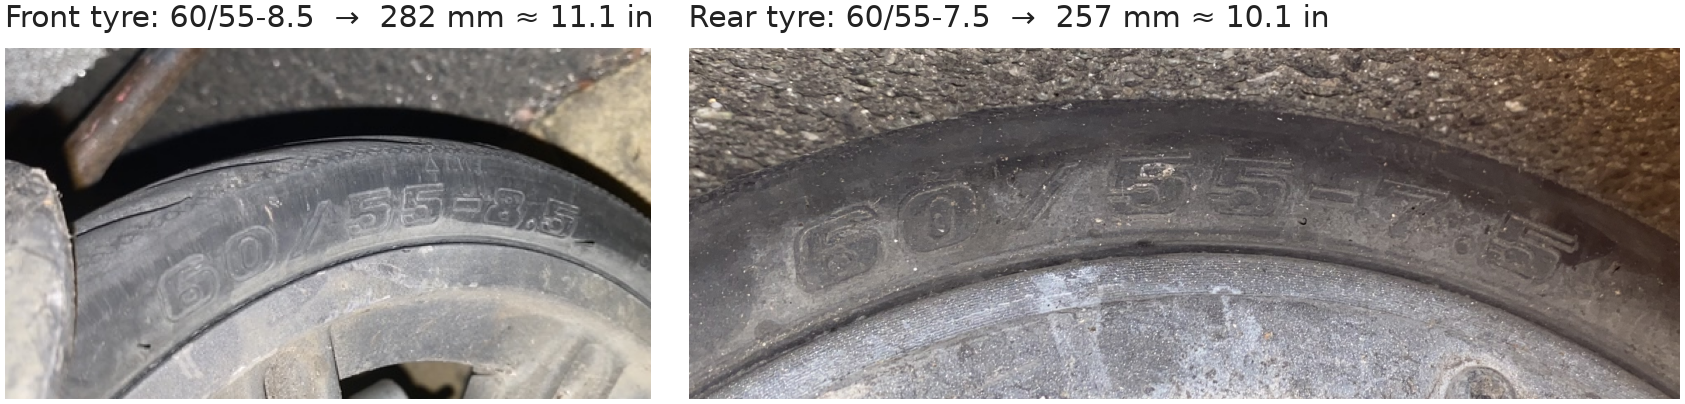
\includegraphics[width=\linewidth]{fig_tyres.png}
\caption{Tyre sidewall size codes of a Voi Voiager 5 parked in Oxford, photographed by the
author on 9 October 2026 (crops). Metric code width/aspect ratio-rim diameter; nominal
outer diameter = rim + 2 $\times$ width $\times$ aspect ratio. The photographed scooter is the
same model as the three ridden scooters (Voiager 5).}\label{fig:tyres}
% The author verified that the photographed scooter is a Voiager 5 (2026-10-10).
\end{figure}

\subsection{Research question and contributions}

This paper asks whether pothole impacts on the Voiager 5 reach levels associated with loss of
stability, and whether a front wheel larger than its current 11~in would reduce them. It
tests a specific
hypothesis that could turn out to be false:

\begin{quote}
Because the front wheel both steers and takes the peak load at impact, enlarging the front
wheel alone gives most of the stability benefit of enlarging both wheels.
\end{quote}

If the hypothesis held, a front-wheel minimum such as London's would capture most of the
benefit of larger wheels, at lower cost than enlarging both. If it failed, for example
because the rear wheel's impact also caused falls, a front-only rule would be insufficient.

The work has two parts. \textbf{Part A} (Section~\ref{measuring-what-riders-experience-on-the-road})
measures what a rider experiences: three legal rides on Voiager 5 scooters in Oxford, recorded
with a handlebar-mounted smartphone, give the number, size and location of sudden vertical
impacts, which are compared with public pothole reports. The recording method itself is checked,
including whether it can tell riding from walking. \textbf{Part B}
(Sections~\ref{methods-modelling-the-effect-of-wheel-size}
and~\ref{results-what-a-larger-front-wheel-would-change}) uses a geometry model and a planar
dynamics model of scooter and rider to compare the current 11/10 wheels with a smaller
10/10 reference, with larger front wheels alone and with larger wheels front and rear. The measured impacts provide a consistency check
for the model, not a validation.

Compared with earlier work, the contributions are: measurement of discrete impacts on a rental
e-scooter in ordinary use, rather than comfort vibration; repeated impacts at the same places
across rides, compared with what the public had reported; and a direct test of whether a
larger front wheel alone performs like larger wheels front and rear. Section~\ref{sec:discussion}
discusses what the results do and do not show and what they suggest for trial rules.
